\section{Filtro Equirriple Parks-McClellan}

Los filtros FIR con el método de ventanas y con muestreo en frecuencia tienen la desventaja de no tener un control preciso sobre las frecuencias críticas ($f_p$ y $f_a$). El método MiniMax o de Parks-McClellan es un método iterativo para encontrar el filtro FIR óptimo con aproximación Chebyschev. El objetivo del algoritmo es minimizar el error en las bandas de paso y de atenuación usando esta aproximación. Se obtiene de esta forma un filtro con ripple parejo en cada banda, característico de Chebyschev.
\par Entonces la respuesta en frecuencia es igual a:
\begin{equation}
  H_o\left(e^{j\omega}\right)=P(\omega).Q(\omega)
\end{equation}
con $P(\omega)=\sum_{k=0}^L\alpha(k)\cos(\omega k)$ y $L=\frac{N-1}{2}$ para \textsc{Tipos I y II} y $L=\frac{N}{2}-1$ para \textsc{Tipos III y IV}.
\par Si $H_d(\omega)$ es la respuesta deseada del filtro, $W(\omega)$ podría ser una función que pondera el error de la aproximación y $E(\omega)$ el error de la aproximación. De esta forma:
\begin{equation}
  E(\omega)=W(\omega)[H_d(\omega)-P(\omega).Q(\omega)]
\end{equation}
Lo que se busca en el algoritmo son los coeficientes $\alpha(k)$ que minimicen $E(\omega)$, es decir, el error, en toda la banda donde se aproxima $H_d(\omega)$ por $H_o\left(e^{j\omega}\right)$. Se pueden conseguir así, filtros multibanda con distinto ripple en cada banda de interés.
\par El resultado se observa en la siguiente figura.
\begin{figure}[H]
  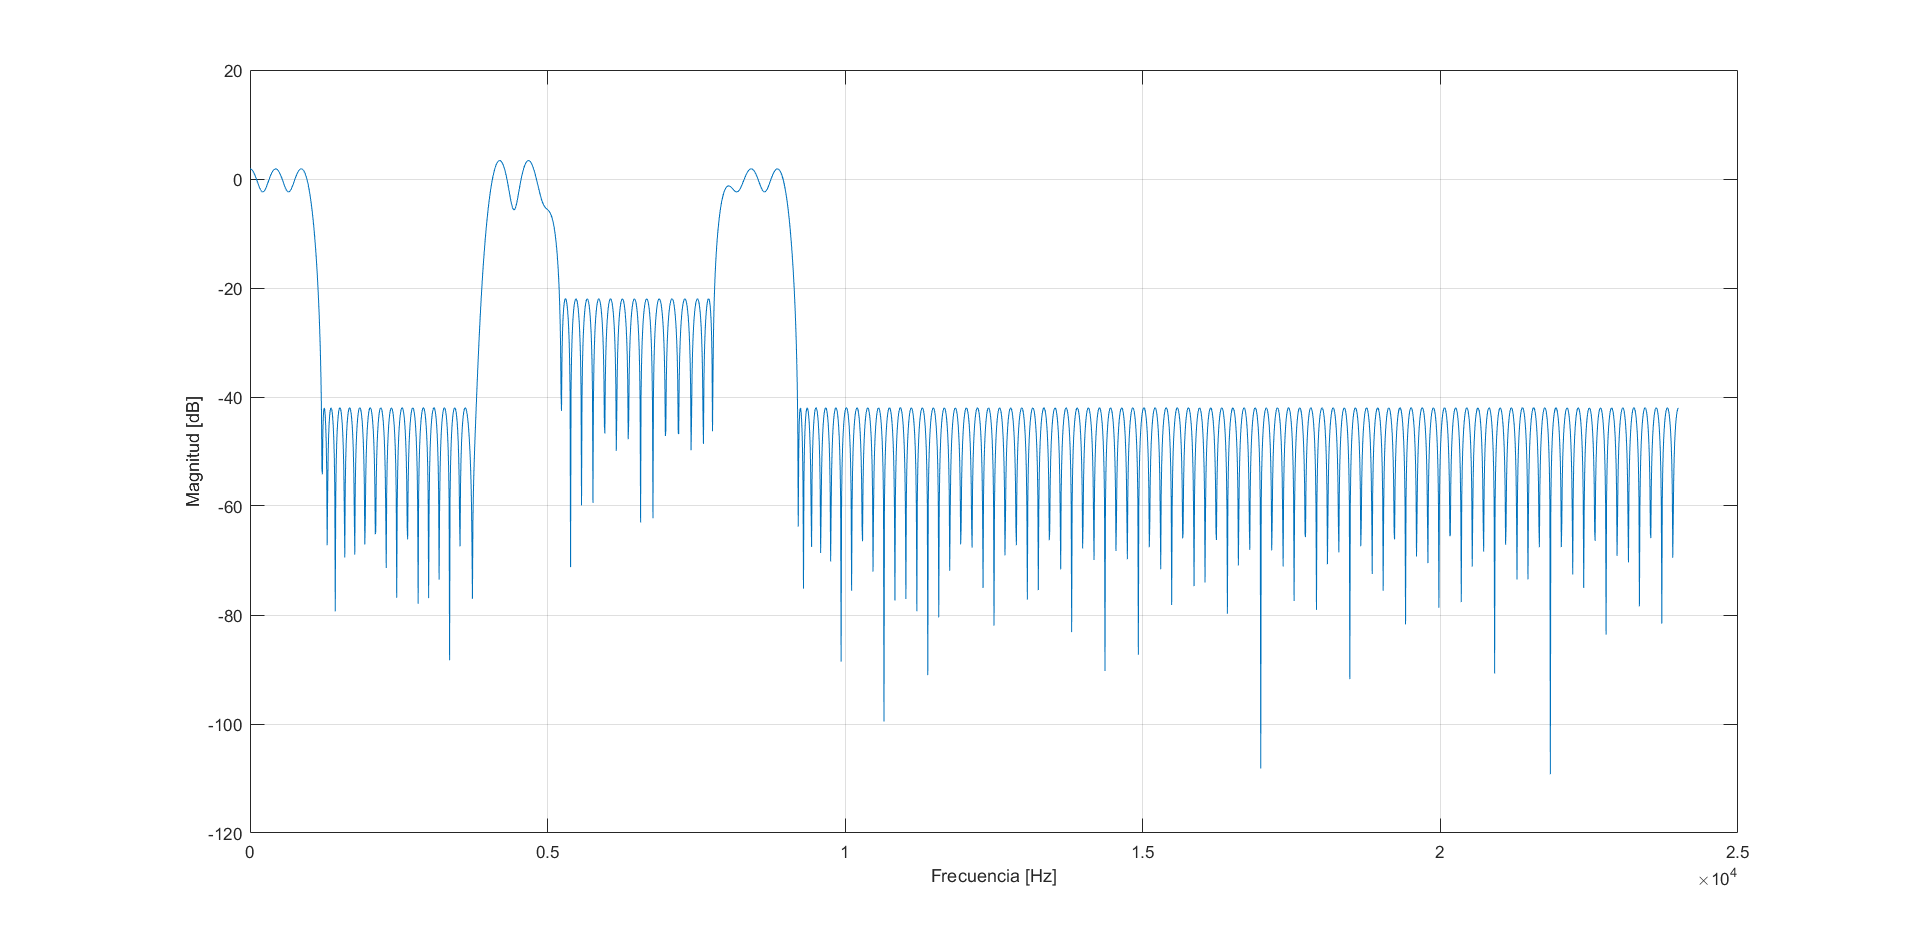
\includegraphics[scale=.35]{./images/4/pm.png}
  \caption{Respuesta en frecuencia del filtro equirriple.}
\end{figure}
A diferencia del método con ventanas, al aumentar el $N$, las mejoras en el ripple se presentaban sólo en zonas sin discontinuidades, en cambio, con el método actual, al aumentar el orden, o la cantidad de muestras $N$, hay mejoras en toda la banda.
